\chapter{Testare și validare}
\pagestyle{fancy}

In acest capitol sunt descrise testele efectuate asupra sistemului de monitorizare a calitatii aerului si rezultatele obtinute in urma acestora. In cadrul fiecarui 
test vor fi prezentate capturi de ecran ale aplicatiei Android continand valorile raportate de senzor si grafice. In capturile de ecran se va observa ca fiecare 
valoare prezentata are o culoare care se modifica pe parcursul testului. Aceasta culoare reprezinta gradul de calitate al aerului:
\begin{itemize}
	\item Verde - Calitatea aerului este foarte buna.
	\item Galben - Calitatea aerului este moderata.
	\item Portocaliu - Calitatea aerului este slaba. 
	\item Rosu - Calitatea aerului este foarte slaba.
	\item Mov - Calitatea aerului este periculoasa.
	\item Maro - Calitatea aerului este extrem de periculoasa.
\end{itemize}

\section{Testare raspuns senzori la schimbarile mediului}\label{sec:tv_environmental_variation}
\subsection{Variatia temperaturii}\label{subsec:tv_temperature_variation}
In acest test temperatura a fost variata de la cea a camerei pana la 55 de grade celsius utilizand o camera termica. S-a ales limita de 55 de grade celsius deoarece 
senzorul de particule in suspensie SPS30 are specificata in fisa de date ca temperatura de functionare maxima 60 de grade celsius.

Pentru compararea valorilor raportate de senzorul HDC1080 a fost utilizat senzorul de temperatura al camerei termice. Acest senzor utilizeaza 3 termocuple de tip T 
pentru raportarea la fiecare minut a temperaturii din camera termica. Valorile raportate sunt reprezentate grafic.

In prima captura de ecran din figura \ref{fig:tv_temp_var_sensor_view}, starea initiala, se observa ca toate valorile prezinta o calitate a aerului buna, exceptand umiditatea care prezinta o calitate a aerului 
moderata. 

In a doua captura de ecran din figura \ref{fig:tv_temp_var_sensor_view}, starea intermediara, se observa cresterea temperaturii la 38.193 grade celsius care prezinta o calitate a aerului periculoasa si scaderea umiditatii 
la 37.615 \% care prezinta o calitate a aerului moderata. Indicii particulelor in suspensie (PM1.0, PM2.5, PM4.0 si PM10.0) si Indicele Compusilor Organici Volatili 
nu au suferit modificari notabile prezentand in continuare o calitate a aerului buna.

In a treia captura de ecran din figura \ref{fig:tv_temp_var_sensor_view}, momentul opririi incalzitorului camerei termice, se observa ca valoarea temperaturii a crescut la 54.115 grade celsius reprezentand un mediu foarte 
periculos. Umiditatea a scazut la valoarea 27.331 \% reprezentand o calitate a aerului slaba. Particulele in suspensie au crescut la valori foarte mari reprezentand un 
mediu foarte periculos, acest lucru poate fi cauzat de elementele camerei termice care incalzite la 55 de grade celsius pot sa degaje particule in aer. Indicele Compusilor 
Organici Volatili (VOCIndex) nu a fost afectat pe intreaga durata a testului.

In graficul de temperatura din figura \ref{fig:tv_temp_var_chart_view} se poate oserva curba de crestere a temperaturii, mentinerea temperaturii de aproximativ 55 de 
grade celsius pentru o perioada de timp si curba abrupta de coborare a temperaturii in momentul in care camera termica a fost deschisa. O comparatie intre graficul de 
temperatura al senzorului de calitate a aerului, figura \ref{fig:tv_temp_var_chart_view}, si graficul senzorului etalon, figura \ref{fig:tv_temp_var_waist_chart} ne 
arata modul in care fiecare senzor a urmarit cresterea si scaderea temperaturii din camera termica. Deoarece temperatura in camera termica a crescut foarte repede senzorul 
etalon a ajuns la un maxim de 62.5 grade celsius in timp ce senzorul de calitate a aerului la 54.115 grade celsius. Dupa o perioada de stabilizare a temperaturii din 
camera termica ambii senzori au raportat temperaturi foarte apropiate in jurul valorii de 54.115 grade celsius. La deschiderea camerei termice, senzorul etalon a detectat 
scaderea brusca a temperaturii mult mai repede decat senzorul de calitate a aerului. Acest lucru este datorat faptului ca senzorul etalon utilizeaza termocuple care sunt 
detasate de placa de circuite integrate, iar temperatura acesteia nu afecteaza temperatura reala. Dupa o perioada de stabilizare in care senzorul de calitate a aerului s-a 
racit, ambii senzori raportau valori foarte apropiate in jurul valorii de 26.6 grade celsius.

Pe perioada testului umiditatea din camera termica a scazut, iar momentul deschiderii camerei termice poate fi observat in graficul de umiditate din figura 
\ref{fig:tv_temp_var_chart_view} prin caderea brusca a umiditatii si imediata crestere a acesteia. Din graficele particulelor in suspensie (PM1.0, PM2.5, PM4.0 si PM10.0) 
se observa ca la trecerea peste 47 de grade celsius senzorul SPS30 a avut o perioada de zgomot in care a raportat valori consecutive foarte mari sau foarte mici, iar apoi 
s-a stabilizat la valori foarte mari care au scazut treptat. Acest lucru poate semnala o eroare a senzorului la temperatura respectiva. In graficul indicelui de 
calitate a aerului (VOCIndex), de asemenea, se poate observa deschiderea camerei termice prin scaderea brusca a acestuia si apoi urcarea catre valorile corecte ale 
mediului ambiental. 

Figura \ref{fig:tv_temp_var_sensor_view} prezinta 3 capturi de ecran din timpul testului reprezentand starea initiala, o stare intermediara si starea din momentul 
opririi incalzitorului camerei termice. 
\begin{figure}[H]
    \centering
    \includegraphics[scale=0.16]{figs/tv_temp_var_sensor_view.png}
    \caption{Valorile indicilor de calitate a aerului in punctele cheie ale testului}
    \label{fig:tv_temp_var_sensor_view}
\end{figure}

Figura \ref{fig:tv_temp_var_chart_view} prezinta 3 capturi de ecran care contin reprezentarea grafica a fiecarui indice de calitate a aerului pe 
intreaga durata a testului.
\begin{figure}[H]
    \centering
    \includegraphics[scale=0.18]{figs/tv_temp_var_chart_view.png}
    \caption{Graficele indicilor de calitate a aerului}
    \label{fig:tv_temp_var_chart_view}
\end{figure}

Figura \ref{fig:tv_temp_var_chart_view} prezinta graficul generat de senzorul camerei termice.
\begin{figure}[H]
    \centering
    \includegraphics[scale=0.3]{figs/tv_temp_var_waist_chart.png}
    \caption{Graficul senzorului etalon}
    \label{fig:tv_temp_var_waist_chart}
\end{figure}

\subsection{Variatia particulelor in suspensie din aer}
Pentru realizarea acestui test senzorul de calitate a aerului a fost amplasat intr-o cutie de carton pentru a limita dimensiunea mediului la care acesta este expus. 
Printr-o gaura in partea superioara a cutiei a fost introdus in mod treptat fum.

In graficele PM1.0, PM2.5, PM4.0 si PM10.0 din figura \ref{fig:tv_pm_var_chart_view} se observa curbele de crestere si scadere a cantitatii particulelor in suspensie 
pe metru cub. Curba de crestere este destul de brusca, desi s-a incercat introducerea de fum in cantitati foarte mici, ceea ce arata sensibilitatea senzorului SPS30. 
Curba de scadere este foarte abrupta si semnifica momentul deschiderii cutiei si automat aerisirea acesteia. In graficul TPS, care reprezinta cantitatea generala a 
partiulelor in suspensie din aer, a crescut pana la valoarea de 700 micrograme pe metru cub, apoi a intrat in saturatie si a raportat valori sub 2 micrograme pe metru 
cub pana cand cutia a fost deschisa si s-a revenit la valori normale. Graficul de temperatura prezinta o crestere pana la 28.6 grade celsius, iar graficul de umiditate 
prezinta o scadere pe durata testului, ceea ce e normal din moment ce in cutie a fost introdus fum cald.    

Figura \ref{fig:tv_pm_var_chart_view} prezinta 3 capturi de ecran care contin reprezentarea grafica a fiecarui indice de calitate a aerului pe 
intreaga durata a testului.
\begin{figure}[H]
    \centering
    \includegraphics[scale=0.16]{figs/tv_pm_var_chart_view.png}
    \caption{Graficele indicilor de calitate a aerului}
    \label{fig:tv_pm_var_chart_view}
\end{figure}

\section{Test de consum de putere}\label{sec:tv_pwrcons}
Pentru realizarea acestui test s-a utilizat un ampermetru legat in serie cu placa de dezvoltare Arty Z7 si o sursa de curent continuu pentru alimentare. Placa de dezvoltare 
poate fi alimentata la 7-15 V prin conectorul J7 pinii VIN si GND si prin amplasarea unui conector jumper in modul REG de pe setul de pini JP5. Astfel, sursa a fost setata 
pe 12 V, firul rosu de iesire din sursa a fost conectat la intrarea ampermetrului, iesirea ampermetrului conectata la pinul VIN de alimentare a senzorului, iar pinul GND 
al senzorului la firul GND al sursei. Acest test ofera punctul de plecare in imbunatatirea consumului senzorului in viitoare versiuni ale acestuia.

Testul a fost efectuat pe o perioada de 30 de minute in care ampermetrul a esantionat valori ale consumului de putere si a facut o medie a acestora, consumul de putere 
rezultat fiind de 151.11 mA/h.

Figura \ref{fig:tv_pwr_cons} prezinta o captura a ecranului ampermetrului unde sunt afisate sub forma grafica valorile esantionate in ultimele 60 de secunde. Perioada 
de esantionare a fost setata pe 0.02 secunde si limitarea de curent la 1 A. In figura se pot observa cateva varfuri in amplitudinea semnalului, acestea reprezinta 
transmisiile radioului. De asemenea, in figura sunt afisate media (151.11 mA/h), maximul (218.9 mA/h) si minimul (139.0 mA/h) consumului de putere detectate in cele 
30 de minute de functionare.
\begin{figure}[H]
    \centering
    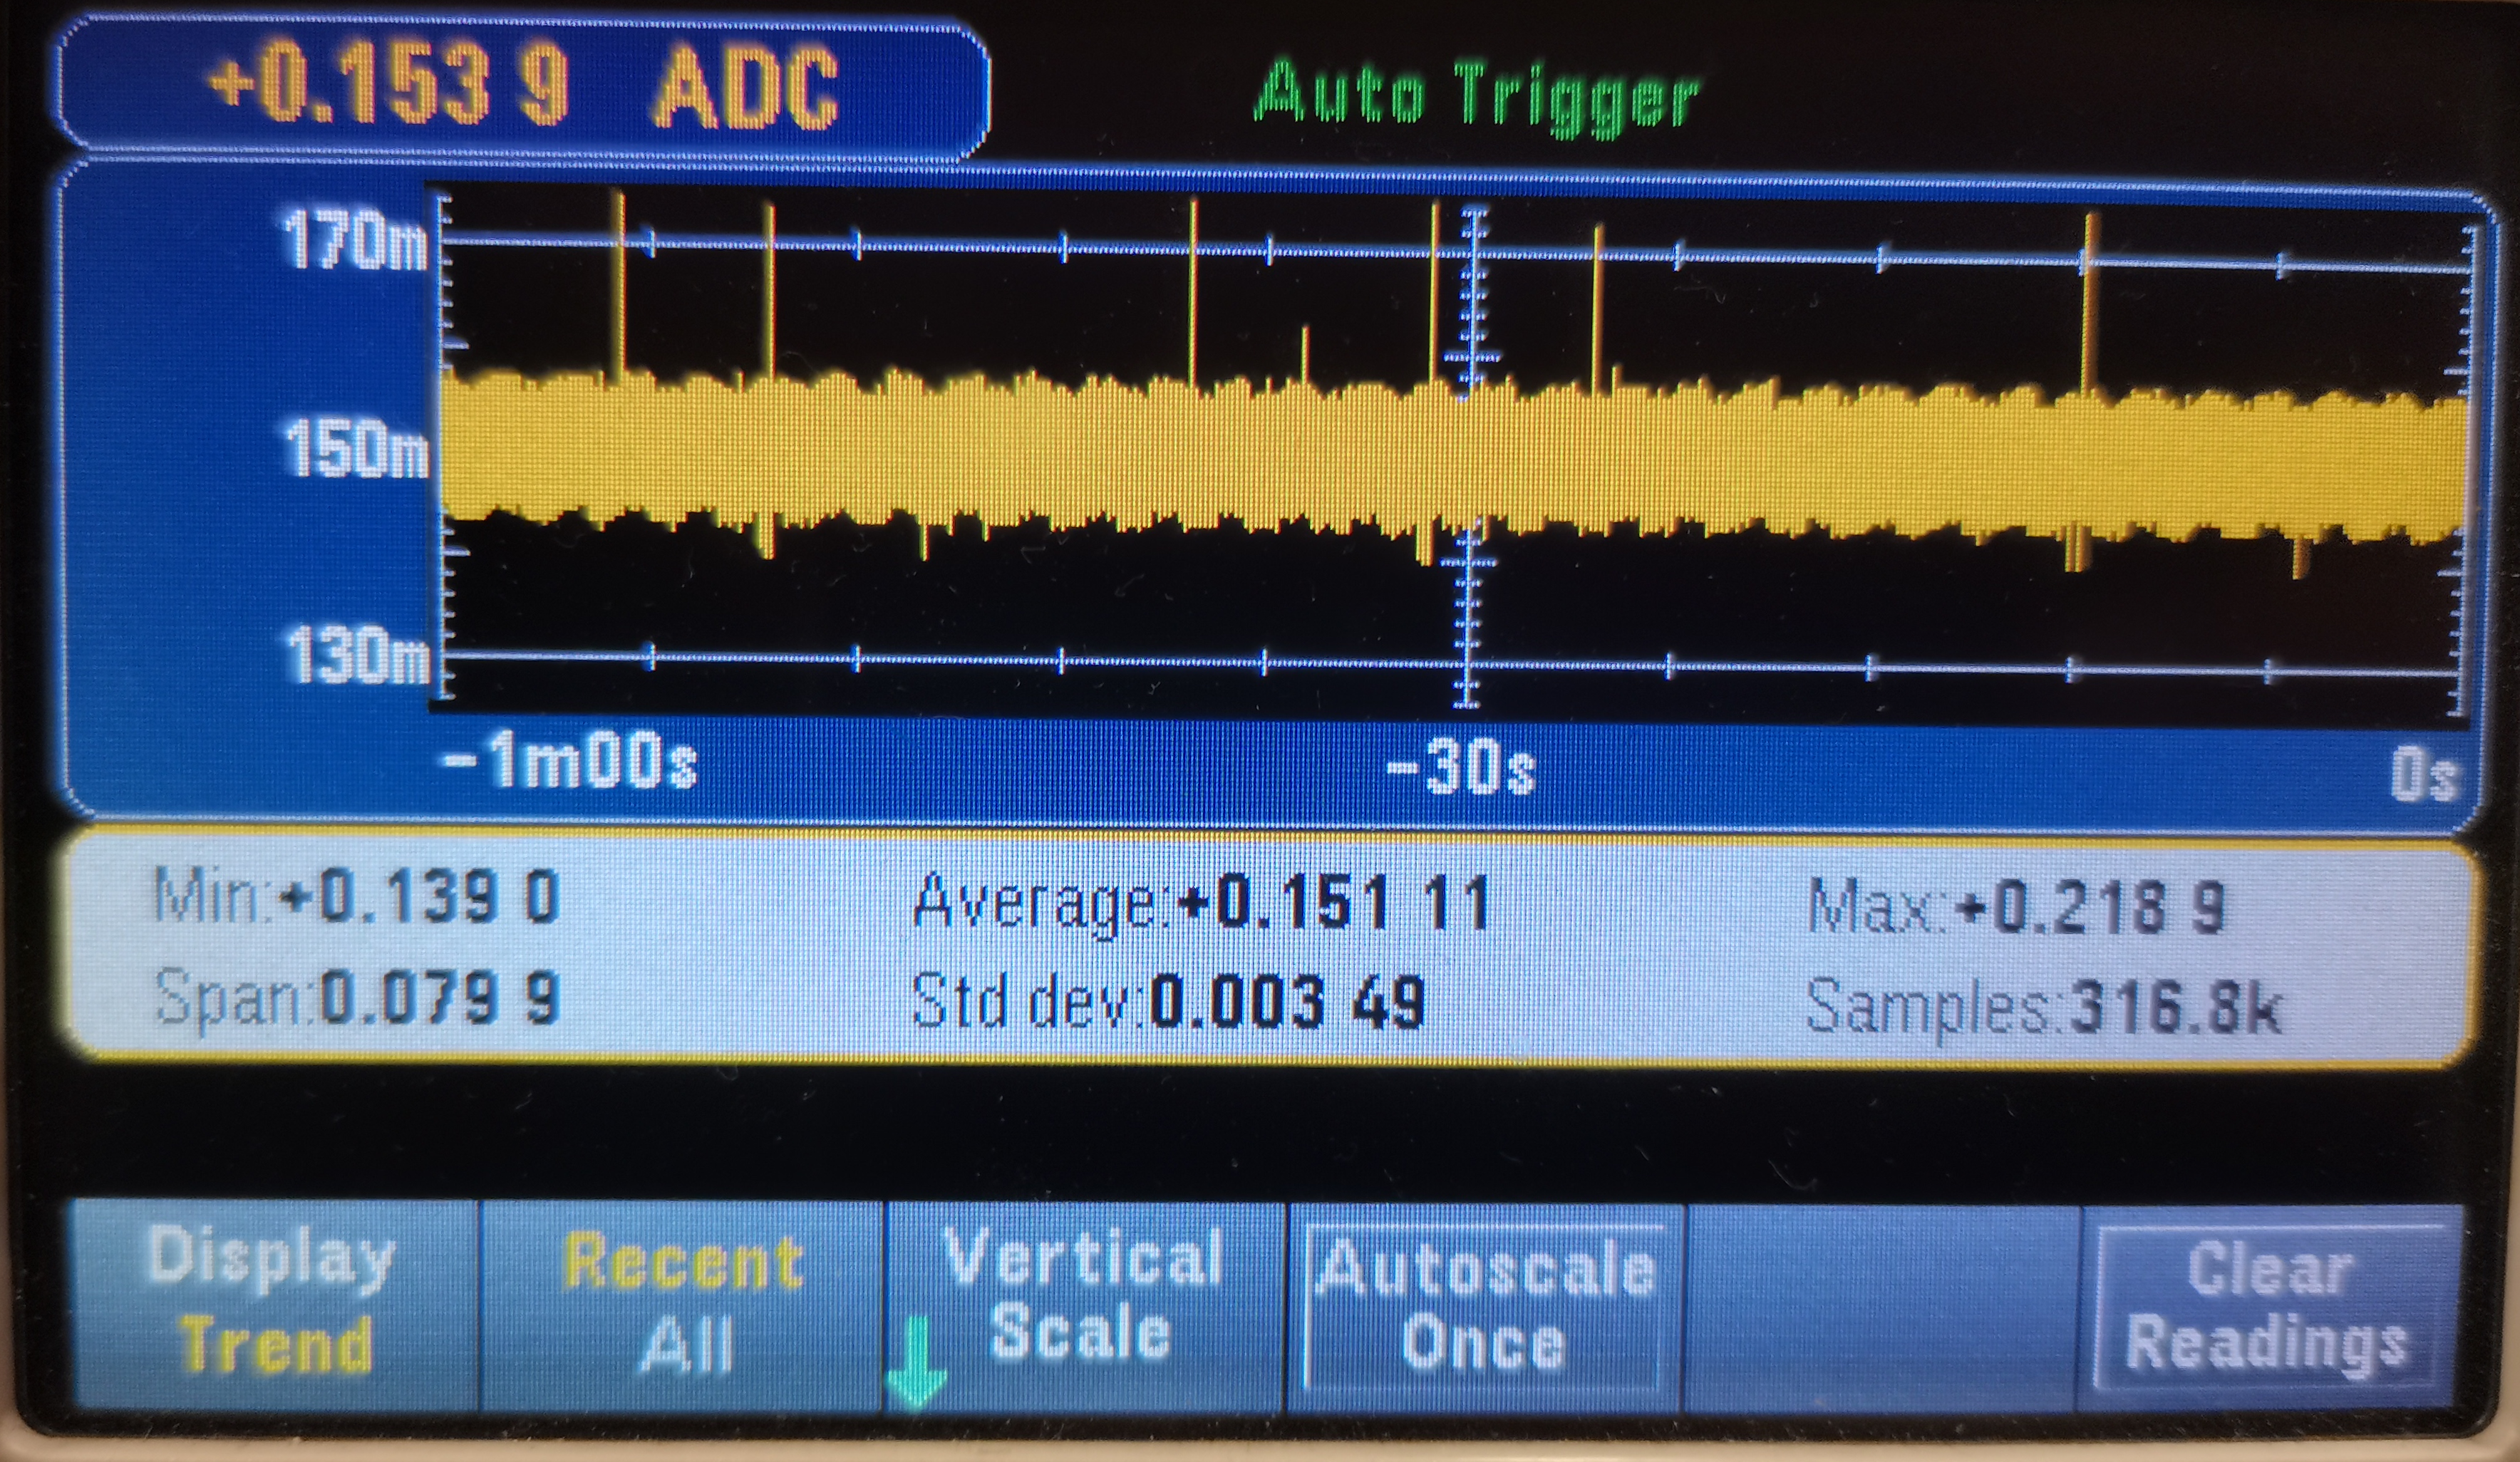
\includegraphics[scale=0.09]{figs/tv_pwr_cons.png}
    \caption{Captura ecran ampermetru digital}
    \label{fig:tv_pwr_cons}
\end{figure}

\section{Scalabilitatea sistemului}\label{sec:tv_scalability}
Acest test are scopul de a demonstra capabilitatea sistemului de monitorizare a calitatii aerului de a gestiona mai multi senzori.

Pentru realizarea testului au fost simulati 20 de senzori utilizand mai multe instante ale unui script scris in limbajul de programare Python. Acest script utilizeaza 
biblioteca Paho MQTT oferita de compania Eclipse sub licenta libera pentru a se conecta la broker-ul MQTT si pentru a publica date cu o periodicitate de 20 de secunde. 
Datele publicate sunt generate prin incrementarea unei variabile inainte de publicarea fiecarui mesaj. Senzorii simulati sunt diferiti de senzorul prezentat in lucrare 
prin faptul ca publica doar date de temperatura si umiditate. S-a ales publicarea acestui set de date pentru a testa capacitatea sistemului de a gestiona un set de date 
diferit si de a valida modificarile care trebuie efectuate cand se doreste utilizarea unui tip de senzor diferit. Pentru crearea mai multor instante a acestui script s-a 
creat un fisier de tip Batch care executa scriptul intr-o bucla care se repeta de 20 de ori. In partea aplicatiei Android, acesti senzori au fost scrisi in memorie ca si 
cum ar fi fost intalati in prealabil. Tipul acestor senzori este "AirQ2", iar tipul senzorului prezentat in lucrare este "AirQ1", acestu lucru se poate observa in prima 
captura de ecran din figura \ref{fig:tv_scalability_welcome_view}. Senzorii simulati au adrese MAC prin care sunt identificati unic incepand de la "000000000001" si pana 
la "000000000020".

In figura \ref{fig:tv_scalability_welcome_view} se poate observa denumirea fiecarui senzor alcatuita din tipul acestuia si ultimele 4 caractere din adresa MAC. Statusul 
conexiunii cu baza de date si cu broker-ul MQTT apare in dreapta fiecarui senzor "Connected". Imaginea senzorilor difera in functie de tipul acestora. 

Testul a fost executat pe o perioada de o ora in care s-a verificat periodic statusul conectivitatii cu baza de date si cu broker-ul MQTT. La finalul testului 
s-a verificat valoarea pe care senzorii o raporteaza. Aceeasi valoare raportata de fiecare senzor inseamna ca nici un pachet nu a fost pierdut. In figura 
\ref{fig:tv_scalability_sensor_chart_view} se poate observa graficul generat pe intreaga perioada de testare.

Figura \ref{fig:tv_scalability_welcome_view} prezinta 3 capturi de ecran reprezentand inceputul, mijlocul si finalul listei senzorilor.
\begin{figure}[H]
    \centering
    \includegraphics[scale=0.16]{figs/tv_scalability_welcome_view.png}
    \caption{Lista senzorilor din aplicatia Android}
    \label{fig:tv_scalability_welcome_view}
\end{figure}

Figura \ref{fig:tv_scalability_sensor_chart_view} prezinta 2 capturi de ecran reprezentand informatiile unuia dintre senzorii simulati, ultimele valori de temperatura 
si umiditate raportate de acestia si graficele pe intreaga durata a testului.
\begin{figure}[H]
    \centering
    \includegraphics[scale=0.18]{figs/tv_scalability_sensor_chart_view.png}
    \caption{Valorile si graficele de temperatura si umiditate la finalul testului}
    \label{fig:tv_scalability_sensor_chart_view}
\end{figure}

\section{Latenta sistemului}\label{sec:tv_latecy}
Acest test are scopul de a calcula cat dureaza ca datele sa ajunga in diferite module ale sistemului de monitorizare a calitatii aerului. Pentru realizarea testului au 
fost adaugate in codul sursa linii de cod care afiseaza timpul curent. In cazul senzorului s-a utilizat un terminal serial care afiseaza momentul de timp cand un mesaj a 
fost receptionat.

Latenta sistemului este impartita in 3 categorii, latenta in cazul datelor in timp real notata T\_real, latenta in cazul datelor istorice notata T\_istoric si 
latenta in cazul salvarii in baza de date notata T\_db.

T\_real este impartita in mai multe puncte si reprezinta durata de timp din momentul inceperii esantionarii datelor si pana la afisareaa acestora pe ecran:
\begin{itemize}
	\item T\_senzor - durata timpului din momentul inceperii achizitiei si pana la transmisia datelor catre aplicatie.
	\item T\_senzor\_app - durata timpului din momentul in care datele au fost transmise catre aplicatie si pana in momentul in care ele au ajuns in aplicatie.
	\item T\_app\_screen - durata timpului din momentul in care datele au intrat in aplicatia Android si pana la aparitia acestora pe ecran.
\end{itemize}

Ecuatia finala este: T\_real = T\_senzor + T\_senzor\_app + T\_app\_screen care este egala cu T\_real = 279ms + 1276ms + 69ms rezultand T\_real = 1.624 secunde 
din momentul inceperii achizitiei si pana la afisareaa datelor pe ecran.

T\_istoric reprezinta durata de timp din momentul in care s-a inceput interogarea bazei de date si pana in momentul in care datele sunt afisate in grafic. Acesta 
poate fi de mai multe feluri in functie de perioada pe care se face interogarea:
\begin{itemize}
	\item T\_istoric\_10m - cazul in care sunt interogate datele din ultimele 10 minute (134 milisecunde).
	\item T\_istoric\_30m - cazul in care sunt interogate datele din ultimele 30 de minute (150 milisecunde).
	\item T\_istoric\_1h - cazul in care sunt interogate datele din ultima ora (176 milisecunde).
	\item T\_istoric\_6h - cazul in care sunt interogate datele din ultimele 6 ore (634 milisecunde).
	\item T\_istoric\_1d - cazul in care sunt interogate datele din ultimele 24 de ore (1.556 secunde).
\end{itemize}

T\_db reprezinta durata de timp din momentul inceperii esantionarii de date si pana in momentul in care datele sunt salvate in baza de date. Acesta este impartit 
in mai multe puncte:
\begin{itemize}
    \item T\_senzor - durata timpului din momentul inceperii achizitiei si pana la transmisia datelor catre aplicatie.
	\item T\_api - durata timpului din momentul in care senzorul a trimis datele si pana in momentul in care datele au fost receptionate de interfata bazei de date.
	\item T\_saved - durata timpului din momentul in care interfata bazei de date a primit cererea HTTP si pana in momentul in care datele au fost salvate in baza 
    de date.
\end{itemize}

Ecuatia finala este: T\_db = T\_senzor + T\_api + T\_saved care este egala cu T\_db = 279ms + 1097ms + 3ms rezultand T\_db = 1.379 secunde 
din momentul inceperii achizitiei si pana la afisareaa datelor pe ecran.

Pe intreaga perioada de testare au fost functionali cei 20 de senzori simulati pentru testul din capitolul \ref{sec:tv_scalability}, deci intervalele de timp 
prezentate in acest capitol au fost esantionate pe o retea de 21 de senzori.